\documentclass[tikz,border=6pt]{standalone}
\usepackage[T1]{fontenc}
\usepackage{lmodern}
\usepackage{amsmath}
\usepackage{amssymb}
\usepackage{bm}
\usepackage{xcolor}
\usepackage{tikz}
\usetikzlibrary{arrows.meta,positioning,fit,calc,backgrounds,shapes.multipart,shapes.geometric}

\colorlet{mandalaBlue}{blue!55!black}
\colorlet{mandalaTeal}{teal!55!black}
\colorlet{mandalaGreen}{green!45!black}
\colorlet{mandalaGold}{orange!70!black}
\colorlet{mandalaRed}{red!55!black}
\colorlet{mandalaViolet}{violet!55!black}
\colorlet{mandalaGray}{black!55}
\colorlet{mandalaLight}{black!3}

\tikzset{
  >=Latex,
  font=\sffamily,
  % Color semantics used consistently across all diagrams:
  % mandalaBlue   -> external inputs / sources / configuration
  % mandalaTeal   -> internal data containers / encoded features
  % mandalaGreen  -> geometric or physics-aware transformations
  % mandalaGold   -> model computation or linear-algebra solve stages
  % mandalaViolet -> predicted operator-valued objects and heads
  % mandalaRed    -> optimization / objectives / losses
  titlebox/.style={
    rounded corners=2.5pt,
    fill=mandalaBlue!8,
    draw=mandalaBlue,
    line width=0.8pt,
    inner sep=6pt,
    minimum height=10mm,
    align=center,
    font=\sffamily\bfseries\large
  },
  panel/.style={
    rounded corners=3pt,
    fill=white,
    draw=black!45,
    line width=0.8pt,
    inner sep=5pt
  },
  stage/.style={
    rounded corners=3pt,
    fill=#1!10,
    draw=#1!85!black,
    line width=0.9pt,
    minimum width=32mm,
    minimum height=11mm,
    align=center,
    font=\sffamily\small
  },
  stage/.default=mandalaBlue,
  smallstage/.style={
    rounded corners=2.5pt,
    fill=#1!9,
    draw=#1!80!black,
    line width=0.75pt,
    minimum width=27mm,
    minimum height=8.5mm,
    align=center,
    font=\sffamily\scriptsize
  },
  smallstage/.default=mandalaBlue,
  sidepanel/.style={
    rounded corners=3pt,
    fill=#1!8,
    draw=#1!75!black,
    line width=0.8pt,
    inner sep=5pt,
    align=left,
    font=\sffamily\scriptsize,
    text width=43mm
  },
  sidepanel/.default=mandalaTeal,
  annot/.style={
    font=\sffamily\scriptsize,
    text=mandalaGray,
    align=left
  },
  arrow/.style={
    -{Latex[length=2.6mm,width=1.8mm]},
    line width=0.95pt,
    draw=black!70
  },
  dashedarrow/.style={
    -{Latex[length=2.4mm,width=1.7mm]},
    line width=0.85pt,
    draw=black!65,
    dashed
  },
  softfit/.style={
    rounded corners=4pt,
    draw=black!35,
    fill=black!1,
    line width=0.7pt,
    inner sep=6pt
  },
  lab/.style={
    font=\sffamily\scriptsize\bfseries,
    text=black!75
  },
  tinycode/.style={
    font=\ttfamily\tiny,
    text=black!70,
    align=center
  }
}

\begin{document}
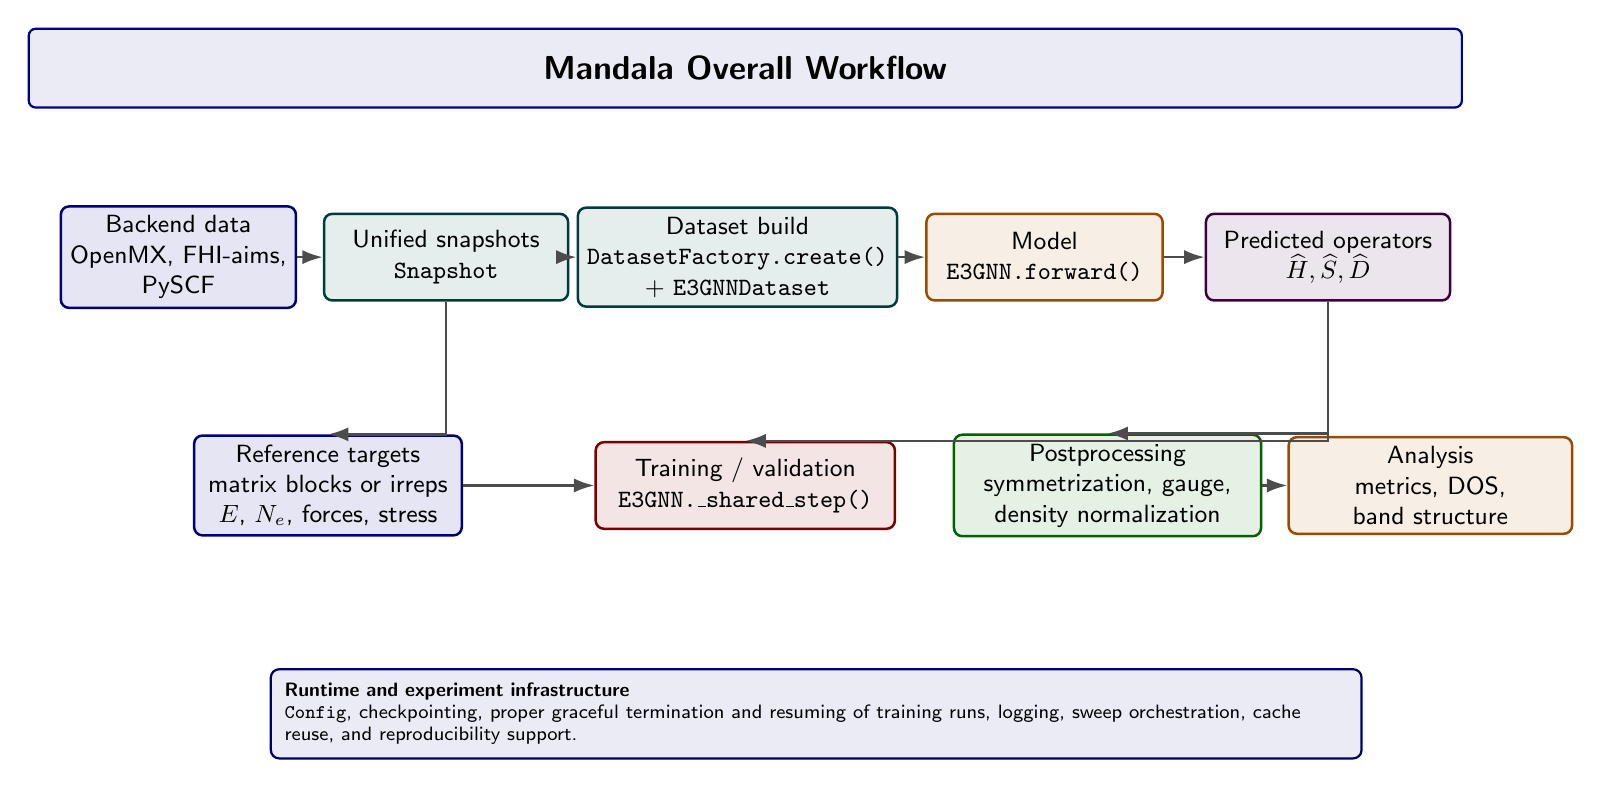
\begin{tikzpicture}[x=1cm,y=1cm]

\node[titlebox, minimum width=18.2cm] (title) at (0,0) {Mandala Overall Workflow};

% Abstract logical schematic:
% (1) backend data -> (2) unified snapshot -> (3) dataset / mapper -> (4) model
% (5) predicted operators feed both training and postprocessing/analysis
% (6) reference targets originate from Snapshot objects
% (7) runtime support stays separate as cross-cutting infrastructure

\node[stage=mandalaBlue, minimum width=2.9cm] (backend) at (-7.2,-2.4)
{Backend data\\OpenMX, FHI-aims,\\PySCF};
\node[stage=mandalaTeal, minimum width=3.1cm] (snapshot) at (-3.8,-2.4)
{Unified snapshots\\\texttt{Snapshot}};
\node[stage=mandalaTeal, minimum width=3.4cm] (dataset) at (-0.1,-2.4)
{Dataset build\\\texttt{DatasetFactory.create()}\\+\ \texttt{E3GNNDataset}};
\node[stage=mandalaGold, minimum width=3.0cm] (model) at (3.8,-2.4)
{Model\\\texttt{E3GNN.forward()}};
\node[stage=mandalaViolet, minimum width=3.1cm] (ops) at (7.4,-2.4)
{Predicted operators\\$\widehat{H},\widehat{S},\widehat{D}$};

\draw[arrow] (backend) -- (snapshot);
\draw[arrow] (snapshot) -- (dataset);
\draw[arrow] (dataset) -- (model);
\draw[arrow] (model) -- (ops);

\node[stage=mandalaBlue, minimum width=3.4cm] (targets) at (-5.3,-5.3)
{Reference targets\\matrix blocks or irreps\\$E$, $N_e$, forces, stress};
\node[stage=mandalaRed, minimum width=3.8cm] (train) at (0.0,-5.3)
{Training / validation\\\texttt{E3GNN.\_shared\_step()}};
\node[stage=mandalaGreen, minimum width=3.9cm] (post) at (4.6,-5.3)
{Postprocessing\\symmetrization, gauge,\\density normalization};
\node[stage=mandalaGold, minimum width=3.6cm] (analysis) at (8.7,-5.3)
{Analysis\\metrics, DOS,\\band structure};

\draw[arrow] (snapshot.south) |- (targets.north);
\draw[arrow] (targets.east) -- (train.west);
\draw[arrow] (ops.south) |- (train.north);
\draw[arrow] (ops.south) |- (post.north);
\draw[arrow] (post.east) -- (analysis.west);

\node[sidepanel=mandalaBlue, text width=13.5cm] (runtime) at (0.9,-8.2)
{\textbf{Runtime and experiment infrastructure}\\
\texttt{Config}, checkpointing, proper graceful termination and resuming of training runs, logging, sweep orchestration, cache reuse, and reproducibility support.};

\end{tikzpicture}
\end{document}
